\section{Types in MiCS} % (fold)
\label{sec:types_in_mics}
	To help understand the core type validation and MiCS type mapping in general its beneficial to realise the different kind of types that are utilized in MiCS.

	\begin{figure}[H]
		\begin{center}
			\centerline{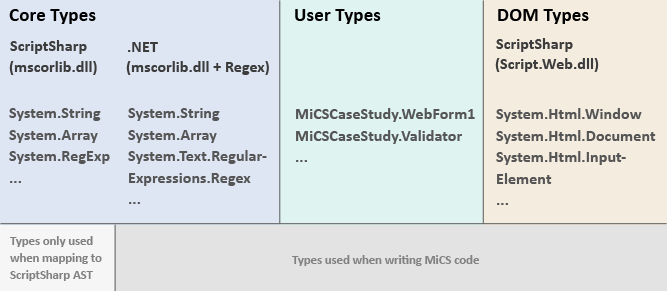
\includegraphics[width=16cm]{resources/images/TypesOverview.png}}
		\end{center}
		\caption{The different kinds of types used in MiCS.}
		\label{typesOverview}
	\end{figure}

	Since one of the goals of MiCS is to be able to execute the same code on both client and server side (server client portability) its required that the .NET core types are used when writing MiCS code. This is in contrast to how Script\# works in its original manner where the Script\# core types (that reflect the equivalent JavaScript types) are used. This has some benefits but is also an obstacle that prevents server client portability. This is because it doesn't make sence to use the Script\# core types when evaluating C\# code in a C\# context (see section \ref{sub:subsection_scriptsharp}).

	\subsection{Core Types} % (fold)
	\label{sub:core_types}
		To build the Script\# AST correctly the Script\# core types are often required to be associated to the AST nodes. One reason that the Script\# core types are required is that they define the type's equivalent script name (in the class attributes). The script name is used by the Script\# script generator. An example is the \texttt{System.Char} (see figure \ref{char}) type which is converted to the JavaScript \texttt{String} type as no JavaScript \texttt{Char} type exists.

	\begin{figure}[H]
			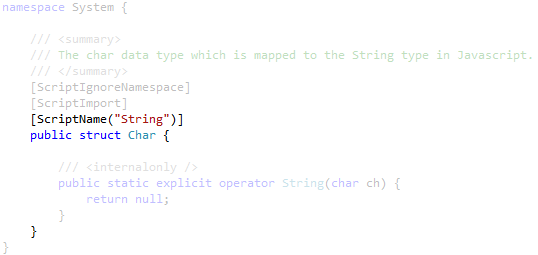
\includegraphics[width=13cm]{resources/images/Char.png}
		\caption{The core type \texttt{System.Char} defined in the Script\# \texttt{mscorlib.dll}.}
		\label{char}
	\end{figure}

		MiCS uses the regular .NET core types when a developer is writing MiCS code but when generating the JavaScript the Script\# defined core types are used. This implies that some kind of mapping between the two kinds of core types are required (explained in section \ref{sub:type_mapping}).
	% subsection core_types (end)

	\subsection{User Types} % (fold)
	\label{sub:user_types}
		User types are the types that are defined by the developer. The user types considered here are either mixed side types or client side types (i.e. types that have method members that have the either the \texttt{MixedSide} attribute or the \texttt{ClientSide} attribute on them). User type definitions is what the generated client side script eventually will consist of. 

		Pure server side types are obviously also user types but they are not relevant in a MiCS context as JavaScript will not be generated from these.
	% subsection user_types (end)

	\subsection{DOM Types} % (fold)
	\label{sub:dom_types}
		Document Object Model (DOM) types are Script\# infrastructure defined in the \texttt{System.Html} namespace (\texttt{Script.Web.dll}). These classes represent DOM objects from the browser. The purpose of these classes is only to represent the interface of the actual DOM types. This is also seen if one looks at the implementation of these types as all their methods and properties return \texttt{null} or \texttt{false}. This emphasizes that it only makes sense to use DOM types for client side only code. Like the Script\# core types, DOM types also has their script names in the attribute \texttt{[ScriptName]}.

		\begin{figure}[H]
				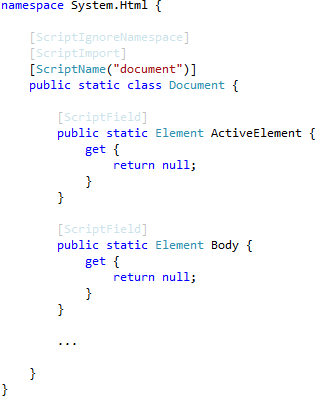
\includegraphics[width=7cm]{resources/images/Document.png}
			\caption{Script\# definition of the DOM type Document.}
			\label{fig:document}
		\end{figure}
	% subsection dom_types (end)

% section types_in_mics (end)